\documentclass[a4paper, 12 pt]{article}

\usepackage[x11names]{xcolor}
\usepackage[top=0.75in, bottom=0.2in, left=0.35in, right=0.35in]{geometry}
\usepackage{graphicx}
\usepackage{booktabs}
\usepackage{url}
\usepackage{enumitem}
\usepackage{palatino}
\usepackage{tabularx}
\usepackage{subcaption}

\newcommand{\coloredSectionDark}[1]{{\small \colorbox{DodgerBlue2}{\begin{minipage}{0.99\textwidth}{\textbf{#1 \vphantom{p\^{E}}}}\end{minipage}}}}
\newcommand{\coloredSection}[1]{{\small \colorbox{DeepSkyBlue1}{\begin{minipage}{0.99\textwidth}{\textbf{#1 \vphantom{p\^{E}}}}\end{minipage}}}}

\begin{document}
\section*{\textcolor{DodgerBlue2}{APRILPROJEKT - KUCHEN BACKEN}}

\noindent
\coloredSectionDark{\textbf{\textcolor{white}{PROJEKTSTATUS}}}\\[-0.3cm]\\
Es gibt 2 wesentliche Projektstatus:\\\\
\noindent
\coloredSection{\textbf{\textcolor{white}{1. PROJEKTSTATUS}}}\\[-0.3cm]\\
Zuerst wird der Teig hergestellt doch bevor das geschieht müssen 2 Vorbereitungen getroffen werden. 
Die Springform muss eingefettet und der Backofen zum Vorheizen angemacht werden. Nun werden die Eier in Eiweiß und Eigelb getrennt.
Anschließend wird das Eiweiß mit etwas Salz steifgeschlagen und ein bisschen Zucker hinzugegeben. Nun wird das Eigelb untergerührt und mit Mehl, Kakao und Backpulver
vermengt. Danach wird die Biskuitmasse in die Springform gefüllt und für 50min in den vorgeheizten Backofen bei 165° C Ober-/Unterhitze
gegeben.\\
Die Füllung wird hergestellt, indem man Kirschen auf einem Sieb abtropft und den Saft auffängt. Von diesem werden 5 EL mit Stärkemehl und etwas Zucker
angerührt. Der restliche Saft wird ebenfalls mit Stärke angerührt und zum Kochen gebracht. Nachdem der Kirschsaft aufbereitet ist, werden die Kirschen wieder zur Füllung hinzugegeben. \\
Die Creme besteht aus Schlagsahne die mit Sahnesteif, Puderzucker und Vanillezucker steifgeschlagen wurde.\\
Die Herstellung der Tränke ist nach dem Vermischen von lauwarmen Wasser mit Kirschwasser bereits abgeschlossen. \\
Nun sind alle Einzelbestandteile des Kuchens hergestellt und für den Zusammenbau der Torte fertig vorbereitet.\\\\
\noindent
\coloredSection{\textbf{\textcolor{white}{2. PROJEKTSTATUS}}}\\[-0.3cm]\\
Die fertige Kuchenmasse wird zuerst zweimal waagrecht durchgeschnitten, wodurch 3 Kuchenschichten entstehen. Die erste bildet den Kuchenboden,
die zweite das Mittelstück und die dritte die oberste Schicht. Im Anschluss wird der Kuchenboden getränkt und daraufhin ein Sahnering auf den Rand des 
Tortenbodens gespritzt. Die abgekühlte Füllung wird nun in der Mitte des Sahnerings aufgetragen und glattgestrichen. \\
Nun wird das Mittelstück ebenfalls getränkt, aufgelegt und mit Sahne bestrichen. Analog verhält es sich auch mit der obersten Kuchenschicht. \\
Im Anschluss wird die Torte noch rundum dünn mit Sahne eingestrichen und mit Schokoraspeln und den Belegkirschen verziert. 
Nachdem der Kuchen nun einige Stunden kaltgestellt wurde ist er bereit für den Verzehr. \\\\
\noindent
\coloredSection{\textbf{\textcolor{white}{ABBILDUNGEN}}}\\[-0.3cm]\\
\begin{figure}[h!]
    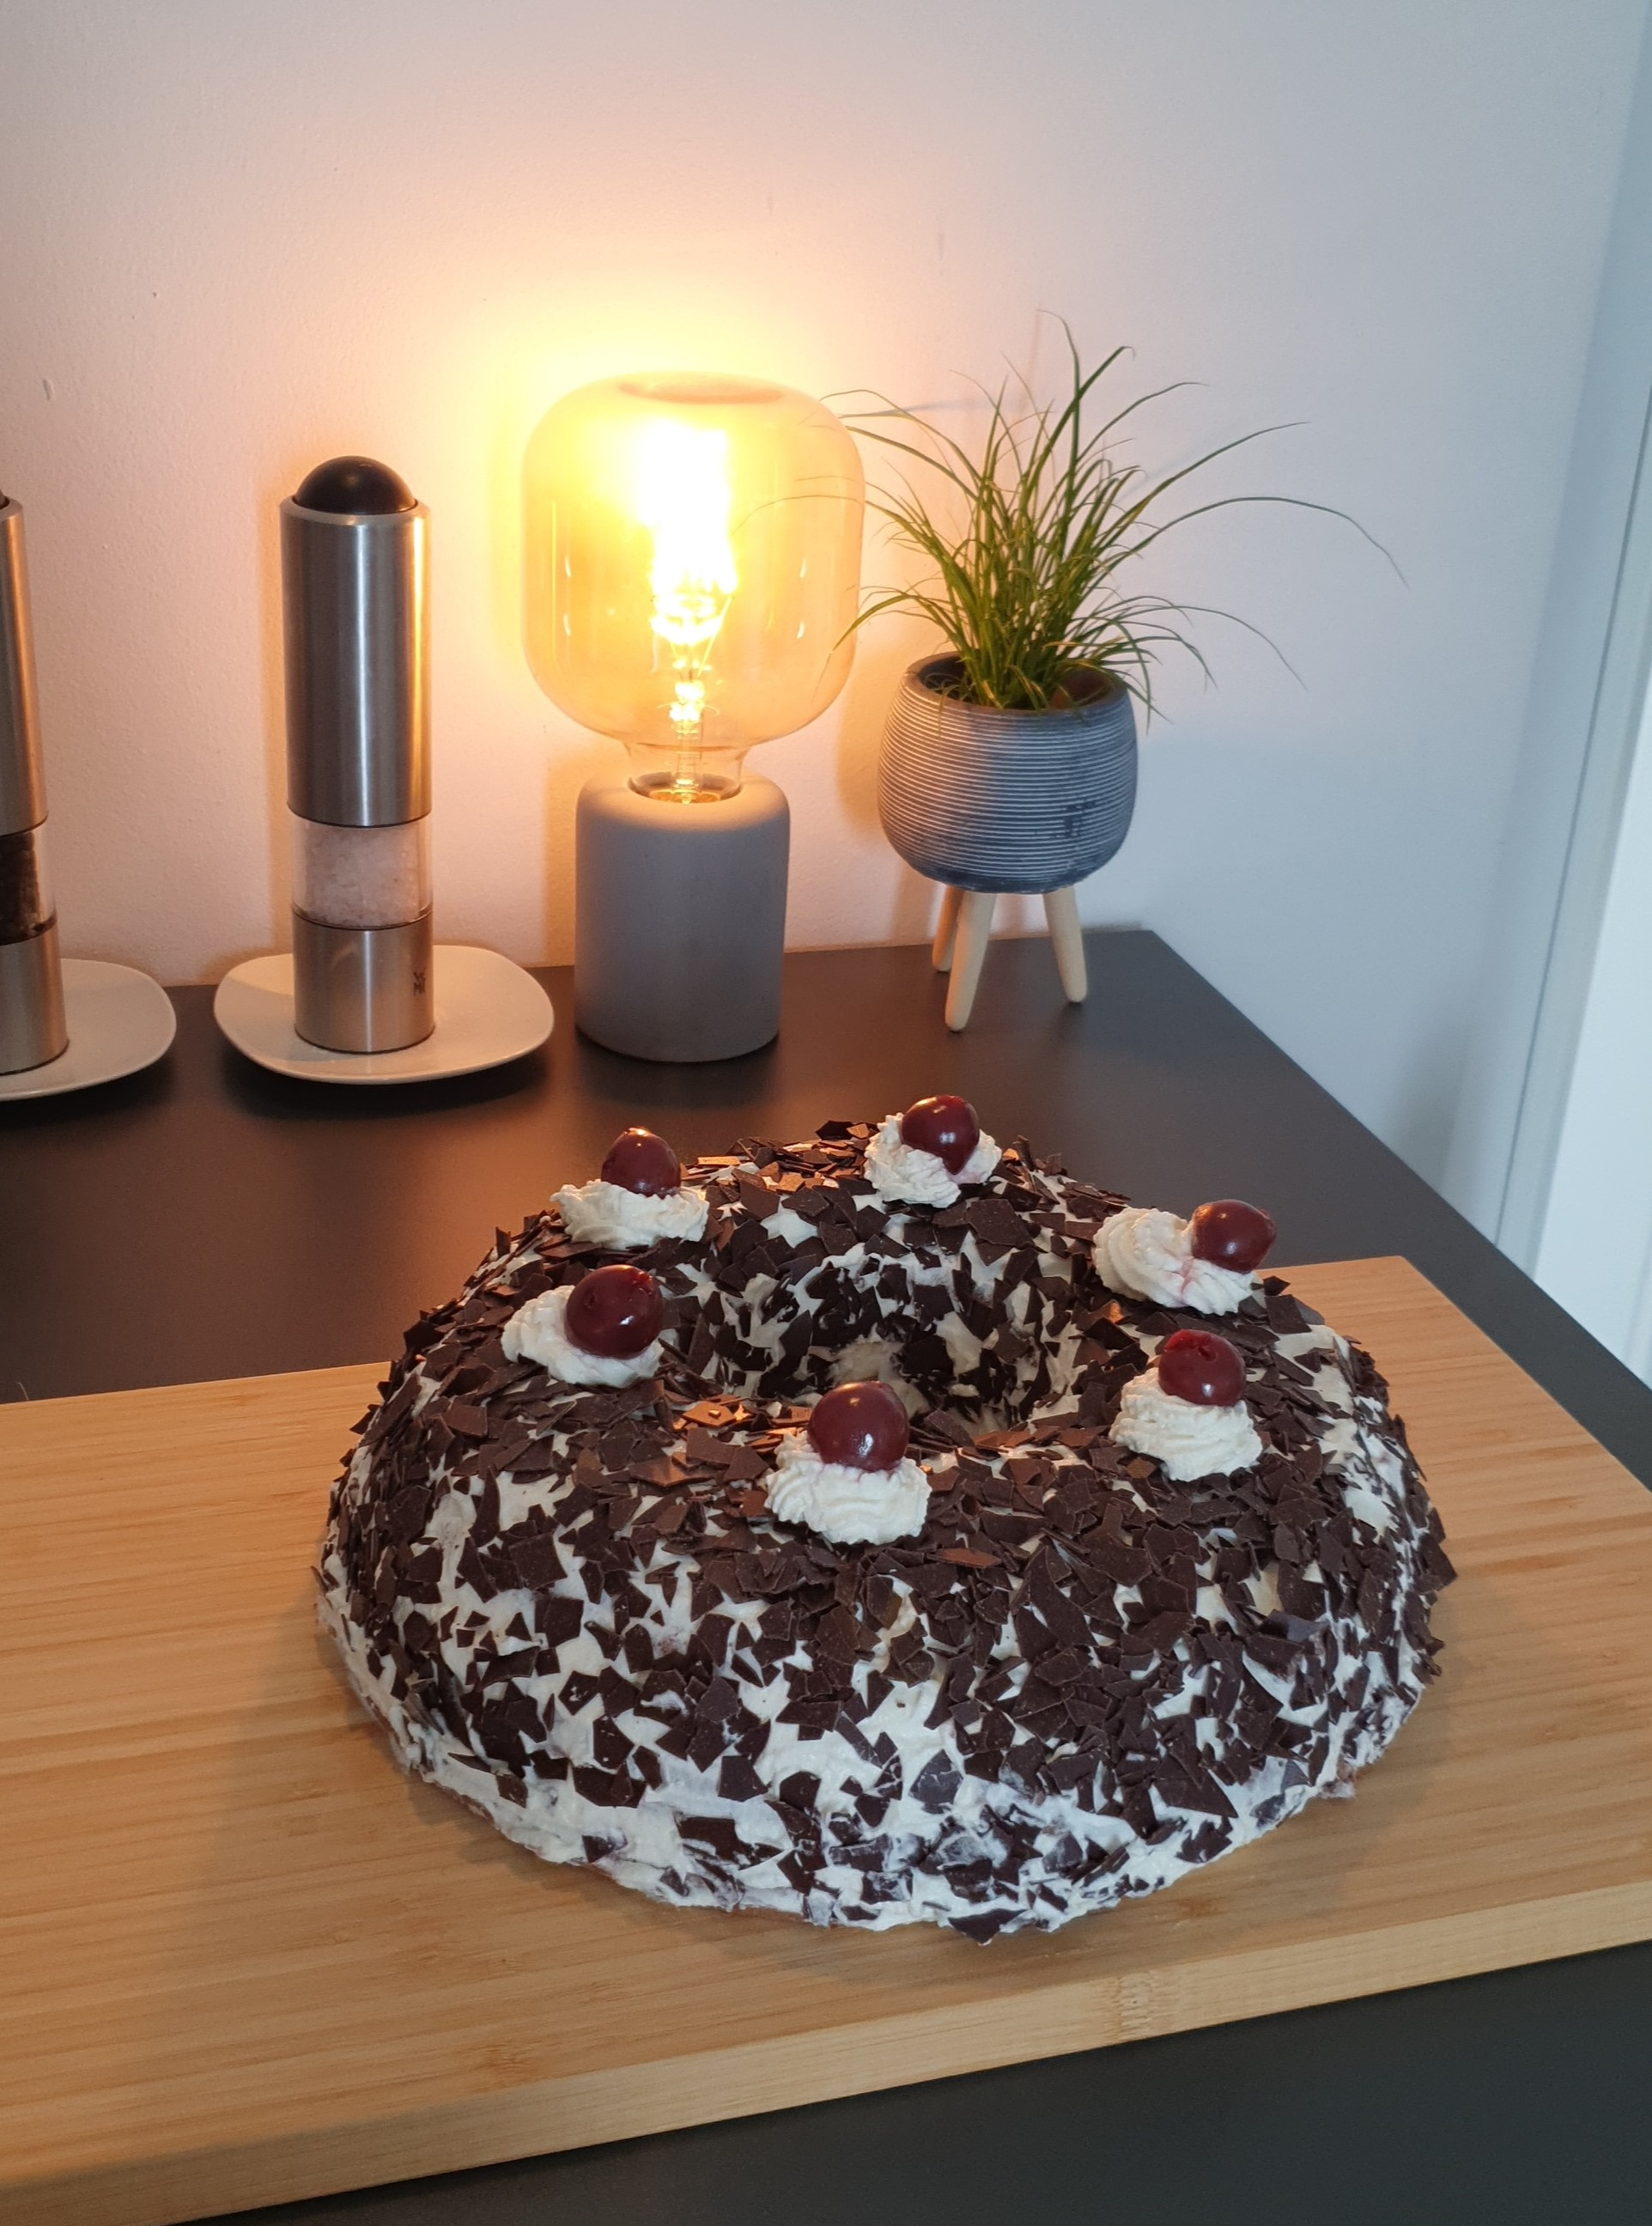
\includegraphics[width=1\linewidth]{FertigerKuchen.jpg}
    \caption{Die fertige Schwarzwälder Kirschtorte}
    \label{fig:cake}
  \end{figure}
\end{document}